\documentclass[10pt,a4paper]{ddedoc}

\usepackage{graphicx}
\usepackage{amsmath,amssymb}
\usepackage{url}
\usepackage{listings}

\pagestyle{plain}

\textwidth=6.25in
\textheight=9.5in
\hoffset=-0.6in
\voffset=-0.8in


\newcommand{\ds}{\displaystyle}

\newcommand{\fun}[1]{{\lstinline!#1!}}

\newcommand{\funp}[1]{{\tt #1}}

% A font for UNIX commands
\newcommand{\commandf}[1]{{\tt #1}}

% A font for environment variables
\newcommand{\envf}[1]{{\it #1}}

% A font for function names
\newcommand{\funcf}[1]{{\bf #1}}

% A font for filenames
\newcommand{\filef}[1]{{\sf #1}}

% A font for ftp sites and web pages
\newcommand{\webf}[1]{{\sl #1}}


\def\pdde{{P\kern-.15emD\kern-.15emD\kern-.15emE\raisebox{.25ex}{-}C\kern-.1emO\kern-.1emN\kern-.05emT}}

\begin{document}
\lstset{language=C++,tabsize=3,columns=flexible,breaklines=true,escapechar=\%}
\makeatother
%
\title{\pdde}
\subtitle{A continuation and bifurcation software for delay-differential equations}
\author{R\'obert Szalai}
\newcommand{\pddever}{0.9.19}
\version{\pddever}
\date{30 September, 2005}
\maketitle

\begin{center}
{\bf \large Revision history } \vskip 0.25em
  \begin{tabular}{ |l|c|l| }
    \hline Date & Version & Institution \\
    \hline Sept.\ 2002 -- Jan.\ 2004 & & Budapest University of Technology and Economics \\
    \hline Febr.\ 2004 -- July 2004 & & University of Bristol \\
    \hline Sept.\ 2004 -- June 2005 & 0.9.2 -- 0.9.8 & Massachusetts Institute of Technology \\
    \hline July 2005 -- Sept. 2005 & 0.9.9 -- 0.9.17 & N.A. \\
    \hline Sept. 2005 -- & 0.9.18 -- & Budapest University of Technology and Economics \\
    \hline
  \end{tabular}
\end{center}

\vskip 3em
\hrule
\vskip 2em
\begin{center} {\bf \large Trademarks } \vskip 0.25em \end{center}
The product names used in this manual are for identification purposes only. All trademarks and registered trademarks are the property of their respective owners.

\newpage

\tableofcontents

\newpage

\section{Introduction}

Several physical, engineering and biological problems require knowledge about dynamical structures and their dependence on parameters in delay-differential equations (see, e.g., \cite{orosz,kirk}). These systems are usually impossible to investigate analytically, so numerical techniques have to be applied. For the first attempt in analyzing the governing equations one usually conducts simulations, which can reveal some information about the invariant structures, particularly about the attractors in the system. However knowing only about the attractors is often insufficient, because unstable structures or repellors form the boundaries of basins of attraction and also can lead to complicated dynamics like chaos. Hence global methods for discovering instabilities are essential.

Continuation techniques provide a tool to discover the parameter dependence of invariant structures. Generally, invariant structures are connected to each other by means of bifurcations, that is, when invariant structures change into or give birth to other structures. In this way, by keeping track of these changes a fairly complete picture can be gained about the global dynamics.

This manual describes the software \pdde, which is capable of continuing periodic orbits and their
bifurcations in delay-differential equations.

\subsection{Capabilities}
\label{capabilities}

The software can handle delay-differential equation in the general form 
\begin{equation}
	\dot{x}(t) = f (t, x(t-\tau_0), x(t - \tau_1), \dots , x(t - \tau_r), \lambda ), \label{gensys}
\end{equation}
where $f(t, \dots ) = f(t + T, \dots)$ is $T$-periodic, $x \in \mathbb{R}^n$ is the dependent variable defined on $I \subset \mathbb{R}$, $\lambda \in \mathbb{R}^p$ is the parameter vector and $0 \le \tau_i$ are positive delays, which can depend on the parameters $\tau_i : \mathbb{R}^p \to [0,\infty)$.
In general $f$ need not depend on $t$, which is called the autonomous case and is handled separately by imposing a so-called phase condition.
The software can continue periodic solutions of (\ref{gensys}), if there is an initial periodic solution available $x_0(t)$ at some parameter value $\lambda_0$. This starting periodic solution has to be specified either in the system definition (C++ source file) or it can be loaded from an input file. The periodic solutions can bifurcate in several ways. If one of the three common one-codimension bifurcations (fold, period doubling, Neimark-Sacker) are found along the branch of periodic solutions, they can be used as starting points for continuing them along two parameters.

\paragraph{Remark.} Fixed points of autonomous systems can be also handled, as periodic solutions of periodic systems by keeping the period constant. Although it is very inefficient, this capability might be useful, when looking for periodic orbits arising at Hopf bifurcations points. Hopf bifurcations of fixed points are detected as Neimark-Sacker bifurcations, and the periodic solutions emanating from such points can be continued by switching to the periodic solution branch using the solution \funp{TYPE=16}. The failure or success of the switch depends on the choice of the period length for the fixed point and the starting solution amplitude \funp{DSSTART}.
As a rule of thumb, the period should be chosen as small as possible to reliably detect the period of the arising periodic orbit. If the period is chosen to be large, the detected period will be some integer multiple of the actual period.

\section{Installation}

The recommended way of compiling the package is to use the GNU C and C++ compilers of versions 3.2.3 and later. Also the Sun Studio 10 compilers can build the package.

\subsection{Linux and Solaris}

The software comes in a compressed archive form \filef{pdde-cont-{\pddever}.tar.gz}, so it has to be unzipped first into an empty directory using the following command.
{ \small \begin{quote} \begin{lstlisting}[basicstyle=\ttfamily,frame=single]
$ gzip -d pdde-cont-%\@version%.tar.gz
$ tar xvf pdde-cont-%\@version%.tar
\end{lstlisting} \end{quote} } \noindent
The software depends on other library packages. Most of them are distributed within the package. However the ATLAS basic linear algebraic software is not included, because it has to be fine tuned for every processor type. Hence, before compiling \pdde\ one has to obtain a recent stable version of ATLAS from \url{http://math-atlas.sourceforge.net}. After compiling the library the resulting archive files (\filef{libatlas.a} and \filef{libcblas.a}) should be copied into the \filef{ATLAS/lib} directory in \pdde 's source tree. These archive files are pre-compiled for various processors so in most cases no compilation step is necessary.

The second step is to configure the package using the \filef{configure} script.
{ \small \begin{quote} \begin{lstlisting}[basicstyle=\tt,frame=single]
$ cd pdde-cont-%\@version%
$ ./configure --prefix=$HOME/pdde-cont/
\end{lstlisting} \end{quote} } \noindent
This generates the platform dependent \filef{Makefile}s and instructs the installer to use \filef{pdde-cont/} as the installation target in the user's home directory. If everything went fine install the software.
{ \small \begin{quote} \begin{lstlisting}[basicstyle=\tt,frame=single]
$ make
$ make install
\end{lstlisting} \end{quote} } \noindent
In order to make the software functioning, the \filef{PATH} environment variables has to be set up. In case of the \filef{bash} shell include the
{ \small \begin{quote} \begin{lstlisting}[basicstyle=\tt,frame=single]
export PATH=$PATH:$HOME/pdde-cont/bin
\end{lstlisting} \end{quote} } \noindent
line into the \filef{.bash\_profile} configuration file in your \filef{HOME} directory. For the C shell (\filef{csh}) insert the following line
{ \small \begin{quote} \begin{lstlisting}[basicstyle=\tt,frame=single]
set path=( $path $home/pdde-cont/bin )
\end{lstlisting} \end{quote} } \noindent
into \filef{.cshrc}. To activate the changes log out and log in again.

\subsection{Windows}

In order to install the software on Windows the MinGW and MinSYS packages have to be installed first (\url{http://www.mingw.org/}). When installing MinGW, check in all the installation options expect those which refer to the source packages. Copy the \pdde\ package file \filef{pdde-cont-{\pddever}.tar.gz} to \filef{c:$\backslash$home$\backslash$$<$username$>$$\backslash$}. Also, the ATLAS linear algebra library is required to build the software. For instructions how to build ATLAS on Windows refer to \url{http://cens.ioc.ee/~pearu/scipy/BUILD_WIN32.html}. Alternatively, there is a compiled ATLAS package at the same web page for Pention 4 processors. If all the prequisites are at hand, start the MSys shell and follow the Linux installation instructions above. The only difference that \filef{.profile} has to be created in your MSys \filef{HOME} directory:
{ \small \begin{quote} \begin{lstlisting}[basicstyle=\tt,frame=single]
$ echo 'export PATH=$PATH:$HOME/pdde-cont/bin' >.profile
\end{lstlisting} \end{quote} } \noindent
After installing the package restart the MSys shell and the software is ready to use.

\subsection{Unix}

The software loads dynamically linked (shared) object files, which describe the system definition. This feature was included into the software in order to avoid recompiling the package, when the system definition changes or to avoid statically linked, large executables, what AUTO uses. However the runtime facility that supports this feature does not exists only on all computing platforms, and they are mostly incompatible with each other. Our implementation chose Linux's way of loading the system definition as shared objects. This method works also on Solaris and possibly on computing platforms too.

\section{Command line arguments}

The software is controlled by the so-called constants file. This file contains
instructions about all the operations done by the software and also specifies the parameters of the numerical methods.
This file can be specified after the \funp{-c} option. If a previous run is continued, an input file should be given using the \funp{-i} option. The output - as a default choice - is written into \filef{out.pdde} if it is not specified otherwise by the \funp{-o} option. The format of the input and output files will be described later in the manual. Also, the program generates an auxiliary file, which contains the parameter values and the solution norms along the computed solution branch.
This file can be selected by the \funp{-b} option if this data is not intended to be written into the \filef{branch} file. The syntax of the command line arguments is illustrated as
{ \small \begin{quote} \begin{lstlisting}[basicstyle=\tt,frame=single]
$ pdde -c <constants-file> [ -i <input-file> [ -o <output-file> ] [-b <branch-file>]]
\end{lstlisting} \end{quote} } \noindent

\section{The constants file}
\label{constfile}

As an example, we included one of the demo problems:
{ \small \begin{quote} \begin{lstlisting}[basicstyle=\tt,frame=single]
sys-glass.so        SYSNAME
120                 LABEL
0 P1 0              TYPE, CP, NPARX, PARX ....
50 4 5 1 1          NINT, NDEG, NMUL, STAB, NMAT
12 12 4 4           NINT1, NINT2, NDEG1, NDEG2 (for torus computations only)
200 -100.0 100.0    STEPS, CPMIN, CPMAX
0.01 0.01 0.01 0.01 DS, DSMIN, DSMAX, DSSTART
1e-4 1e-4 1e-7      EPSC, EPSR, EPSS
12 12 12            NITC, NITR, NITS
\end{lstlisting} \end{quote} } \noindent
In the first separated column are the parameter values, while the second column refers to their meaning. 
When this file is read the program interprets only the first half of each line, that is, it moves to the next line
after all the necessary parameters are read. Although the rest of the line is simply ignored, 
it is useful to keep the mnemonics of the parameters there. The meaning of the parameters are as
follows.
\begin{description}
\item[\funp{SYSNAME}] ~\\
The name of the shared object file,
which contains the system definition. It is the compiled version of a C++
code. For details see section \ref{sysdef}.
%
\item[\funp{LABEL}] ~\\
The solution label in the input file. The program continues this
solution. If \funp{LABEL}=0 it uses the default solution given in the system
definition file.
%
\item[\funp{TYPE}] ~\\
Specifies the type of the solution to be continued. (The numbers in the parentheses after the description denote the required number of additional free parameters.) For time-periodic systems:
\begin{description}
\item[\funp{0} -] Continuation of periodic solutions (0).
%
\item[\funp{1} -] Continuation of fold bifurcations in two parameters (1). The input is a periodic solution at a fold bifurcation point. The software first generates a starting point, that is, it tries to converge to the fold point using a secant method. After the fold point is found with a good accuracy (see \funp{EPSS}), the tangent of the fold curve is computed so that the continuation can start. All the bifurcations are started in this way.
%
\item[\funp{2} -] Continuation of period-doubling bifurcations (1).
%
\item[\funp{3} -] Continuation of Neimark-Sacker (secondary Hopf) bifurcations (1).
%
\item[\funp{4} -] The software first switches to the period-2 branch at a period doubling bifurcation point
(-1 multiplier) and then follows the arising orbits (0). The switching is done by computing the critical eigenfunction $\varphi^{cr}$. The new solution becomes $x_0(t) = x^{cr}(2\,t)$ and similarly, the tangent of the solution $x'(t) = \varphi^{cr}(2\,t)$. Finally, the tangent is re-normed to norm 1, and the continuation can start.
%
\item[\funp{5} -] Switches to the other solution at a branching point and follows the orbits (0). Similar to \funp{TYPE=1}, first the software converges to the critical solution. Then it computes the critical eigenfunction $\varphi^{cr}$, which will become the tangent of the new branch, so that the continuation can start.
\end{description}
In the case of autonomous systems, the bifurcation continuations and branch switching are started in the same way, the only difference is the inclusion of the phase-condition and a different defining system for fold bifurcations.
\begin{description}
\item[\funp{10} -] Continuation of periodic solutions in autonomous systems (1). The additional parameter is usually the period length \funp{P0}.
%
\item[\funp{11} -] Continuation of fold bifurcations in two parameters (2).
%
\item[\funp{12} -] Continuation of period-doubling bifurcations (2).
%
\item[\funp{13} -] Continuation of Neimark-Sacker (secondary Hopf) bifurcations (2).
%
\item[\funp{14} -] The software first switches to the period-2 branch at a period doubling bifurcation point
(-1 multiplier) and then follows the arising orbits (1).
%
\item[\funp{15} -] Switches to the other solution at a branching point and follows the orbits (1).
%
\item[\funp{16} -] Switches to a periodic solution arising in a Hopf bifurcation point. The input is a constant solution, which represents a fixed point (1). For detailed description see the Remark in Sect.\ \ref{capabilities}.
\end{description}
The software can also continue invariant tori arising at Neimark-Sacker bifurcation points. To continue these quasi-periodic orbits use the following parameters when restarting from Neimark-Sacker points.
\begin{description}
\item[\funp{20} -] In the case of time-periodic systems
%
\item[\funp{30} -] In the case of autonomous systems.
\end{description}
If none of the above apply to a problem, it is possible to specify the set of equations and variables used in continuation, by setting the \funp{TYPE} to \funp{-1}. For details, see the end of this section.
%
\item[\funp{CP}] ~\\
It defines the main continuation parameter. The parameters always start with the letter `\funp{P}', if they are user defined or with `\funp{I}' if they are internal parameters, such as the argument of the characteristic multiplier or
the rotation number of a quasiperiodic orbit.
% (Recognition of internal parameters is not yet implemented, however the can be specified using ordinary parameters. E.g., if \funp{NPAR} is the number of ordinary parameters then an interal parameter is equivalent to P(\funp{NPAR} + internal parameter number)). 
These  internal parameters are
\begin{description}
\item[\funp{I0} -] The argument of the characteristic multiplier in the case of Neimark-Sacker bifurcation continuation. 
\item[\funp{I1} -] The smallest eigenvalue of the characteristic matrix. This is used only when the software constructs a starting point in case of bifurcation continuation or when switches solution branches. (Do not use this!)
\item[\funp{I2} -] It refers to the rotation number of a two-torus. Usually this is kept constant in order to avoid phase-locking.
\end{description}
%
\item[\funp{NPARX}] ~\\
Specifies the number of required additional parameters. This must coincide with the expected value (see \funp{TYPE}).
%
\item[\funp{PARX}] ~\\
A sequence of numbers specifying the additional parameters. In
the case of autonomous problems either \funp{CP} or this should include \funp{P0}, which refers to the period length.
%
\item[\funp{NINT}] ~\\
Number of collocation intervals; heavily depends on the problem.
%
\item[\funp{NDEG}] ~\\
Degree of polynomials used in collocation. Usually 4 or 5.
%
\item[\funp{NMUL}] ~\\
The number of Floquet multipliers to be computed.
%
\item[\funp{STAB}] ~\\
If zero, stability is not computed along the branch. In any case, \funp{NMUL} must have a reasonable value, because the eigenvalues are used when computing the argument angle of the critical multiplier when starting a Neimark-Sacker bifurcation continuation.
%
\item[\funp{NMAT}] ~\\
This is the ration of the maximum delay and the period length, more precisely, the smallest integer such that $\funp{NMAT} \ge \tau_{MAX}/T_{MIN}$.
%
\item[\funp{STEPS}] ~\\
Maximum number of steps on the solution branch.
%
\item[\funp{CPMIN}, \funp{CPMAX}] ~\\
Currently not referenced, just write two numbers.
%
\item[\funp{DS}] ~\\
Starting value of the stepsize in the pseudo-arclength continuation.
It should be reasonably small depending on the problem. \funp{DS} is corrected in every continuation step between its minimum and maximum value. If the Newton method exceeds \funp{NITC} iterations and \funp{DS} reached its minimum value, the continuation is stopped.
%
\item[\funp{DSMIN}, \funp{DSMAX}] ~\\
The minimum and maximum value of \funp{DS}.
%
\item[\funp{DSSTART}] ~\\
Used at branch switch from fixed point to periodic solution and periodic solution to torus. The initial solution is approximated linearly, by adding the linear guess multiplied by \funp{DSSTART} to the fixed point or periodic solution. This guess is in fact the tangent vector of the emanating solution and has unit norm.
%
\item[\funp{EPSC}] ~\\
Convergence tolerance to a periodic solution during continuation. For periodic orbit continuation it is about $10^{-5} - 10^{-6}$, for continuation of bifurcations it can be a bit larger about $10^{-4}$ to achieve reasonable stepsizes (\funp{DS}).
%
\item[\funp{EPSR}] ~\\
Tolerance in the refinement of solutions. (Solution refinement is used only before continuation starts.) It should be less than or equal to \funp{EPSC}.
%
\item[\funp{EPSS}] ~\\
Tolerance of \funp{CP} in converging to a bifurcation point. (Used at branch switching.)
%
\item[\funp{NITC}] ~\\
Maximum number of Newton iteration steps in continuation.
%
\item[\funp{NITR}] ~\\
Maximum number of Newton iteration steps, when converging to an initial solution.
%
\item[\funp{NITS}] ~\\
Maximum number of continuation steps, when finding a bifurcation point using a secant method.
The Newton iterations within a continuation step is controlled by \funp{NITC}.
%
\end{description}

\subsection{User defined equations}
If the \funp{TYPE} constant equals \funp{-1}, the third line of the constants file is different. For example
{ \small \begin{quote} \begin{lstlisting}[basicstyle=\tt,frame=single]
sys-glass.so							SYSNAME
0											LABEL
-1 P2 0 3 E1 E0 E24 3 S1 S0 P0	TYPE, CP, SWITCH, NEQN, EQN[], NVAR, VAR[]
...
\end{lstlisting} \end{quote} } \noindent
specifies three equations and three variables, but the second equation and variable are just placeholders. The first equation \funp{E1} is for the periodic solution \funp{S1}. The third equation \funp{E24} is the phase condition of autonomous systems while the third variable is the period \funp{P0}. The detailed descriptions of possible paramters are as follows.
\begin{description}
\item[\funp{CP}] ~\\
	The continuation parameter, same as above.
%
\item[\funp{SWITCH}] ~\\
	The software switches to another branch of solutions if it is non-zero.
\begin{description}
\item[\funp{0} -] No switch.
\item[\funp{1} -] Switches to the other branch at a branching point. %(I hope it knows which one is which...)
\item[\funp{2} -] Switches to the period-two branch at a period doubling bifurcation.
\item[\funp{3} -] Switches to a quasi-periodic torus at a Neimark-Sacker bifurcation.
\end{description}
\item[\funp{NEQN}] ~\\
	Number of equations. The first equation is always the periodic solution, 
	while the second equation is either the characteristic matrix or not defined.
\item[\funp{EQN}] ~\\
	A sequence of numbers, specifying the equations.
\begin{description}
\item[\funp{E0} -] No equation. It is a placeholder for the second equation if there is no bifurcation continuation.
\item[\funp{E1} -] Periodic solution. This is always the first equation and can occur only there.
\item[\funp{E8} -] Characteristic matrix for fold bifurcation. It can occur only at the second place, like all the characteristic matrices below.
\item[\funp{E9} -] Characteristic matrix for period doubling bifurcation.
\item[\funp{E10} -] Characteristic matrix for Neimark-Sacker bifurcation.
\item[\funp{E11} -] Characteristic matrix for fold bifurcation in autonomous systems.
\item[\funp{E16} -] Equation for keeping the norm of the eigenvector constant. It it necessary in fold and period doubling cases.
\item[\funp{E17} -] Equation for keeping the real part of the norm of the eigenvector constant in case of \funp{E10}.
\item[\funp{E18} -] Equation for keeping the imaginary part of the norm of the eigenvector constant in case of \funp{E10}. Note that both \funp{E17} and \funp{E18} are necessary to continue Neimark-Sacker bifurcations.
\item[\funp{E24} -] Phase condition for autonomous systems.
\item[\funp{E25} -] Phase condition for systems with additional symmetry. (For details, see \cite{haegeman}.)
\item[\funp{E32} -] Quasiperiodic solution on a torus.
\item[\funp{E40} -] The first phase condition for the torus. This is applied only in the case of autonomous equations.
\item[\funp{E41} -] The second phase condition for the torus. It is always necessary.
\end{description}
\item[\funp{NVAR}] ~\\
	Number of free variables. This must equal to the number of equations. Similarly, the first variable is always the periodic solution, the second is either not specified or the kernel vector of the characteristic matrix.
\item[\funp{VAR}] ~\\
	A sequence of numbers, specifying the free variables. A variable can be one of the three types. The starting letters are \funp{S}, \funp{P} or \funp{I}, referring to a system variable, parameter or internal variable, respectively. (For parameters and internal variables see the description of \funp{CP}.) The system variables are defined as follows.
\begin{description}
\item[\funp{S0} -] No variable. Similar to \funp{E0}, this is a placeholder if no kernel vector is computed.
\item[\funp{S1} -] Periodic solution.
\item[\funp{S8} -] The kernel of the characteristic matrix.
\item[\funp{S32} -] Quasi-periodic solution.
\end{description}
In the case of an equation with additonal symmetry, when \funp{E25} is specified, also the symmetric components of the solution has to be declared.
The declaration is the last line of the constants file and contains which parts of the solution are complex. The first number is the number of complex solutions,
while the further numbers are the real and imaginary components in the solution vector. For example
{ \small \begin{quote} \begin{lstlisting}[basicstyle=\tt,frame=single]
...
12 12 12            NITC, NITR, NITS
2 0 1 3 4           NSYM, R0, I0, R1, I1
\end{lstlisting} \end{quote} } \noindent
specifies two symmetric components, where the first complex variable has its real and imaginary parts in the zeroth and first component of the solution vector.
Similarly the second rotational symmetric complex solution component has its real and imaginary part in the third and forth component of the solution vector.
\end{description}


\section{Structure of the output file}

The output file contains all the computed information of a periodic solution 
branch. Also, this file can be used to restart the continuation from a point 
on a branch. The above defined restart \funp{LABEL} refers 
to the number of a line in this file. The structure of a line is described 
in Table \ref{iostruct}.
\begin{table}
\begin{tabular}{|c|c|l|}
\hline
Starting & Length & Content\\
Column & & \\
\hline
1             & 1       & \begin{minipage}[c]{0.5\linewidth} \funp{NPAR}, the number of parameters. It may include internal parameters. \end{minipage}\\
\hline
2             & \funp{NPAR} & Values of parameters\\
\hline
\funp{NPAR}+2  & 1       & \funp{NMUL}: number of Floquet multipliers\\
\hline
\funp{NPAR}+3  & $2\times$\funp{NMUL} & \begin{minipage}[c]{0.5\linewidth} The Floquet multipliers. ( Re($\lambda_1$), Im($\lambda_1$), ..., Re($\lambda_{NMUL}$), Im($\lambda_{NMUL}$) ) \end{minipage} \\
\hline
\funp{NPAR}+$2\times$\funp{NMUL}+3
              & 1       & \begin{minipage}[c]{0.5\linewidth} \funp{NDIM}: dimesion of the right-hand-side function $f$ \end{minipage}\\
\hline
\funp{NPAR}+$2\times$\funp{NMUL}+4 & 1       & \funp{NINT}: number of collocation intervals\\
\hline
\funp{NPAR}+$2\times$\funp{NMUL}+5 & 1       & \funp{NDEG}: degree of collocational polynomials\\
\hline
\funp{NPAR}+$2\times$\funp{NMUL}+6 & \funp{NINT}$\times$\funp{NDEG}+1 & Mesh of the $[0,1]$ interval. \\
\hline
\begin{minipage}{0.2\linewidth} \begin{center}
\funp{NPAR}+$2\times$\funp{NMUL}+\\
\funp{NINT}$\times$\funp{NDEG}+7
\end{center} \end{minipage} & 
\funp{NDIM}$\times$(\funp{NINT}$\times$\funp{NDEG}+1) & 
\begin{minipage}[c]{0.5\linewidth} The solution profile, a sequence of \funp{NDIM}-tuples \end{minipage} \\
\hline
\end{tabular}
\caption{The structure of a line of the input/output files.}
\label{iostruct}
\end{table}

It is possible to convert the solution profile form DDE-BIFTOOL to this format and back. For this use the matlab files \filef{dde2pdde.m} or \filef{pdde2pdd.m} in the \filef{matlab} subdirectory in the following way. Assume that there is branch of periodic solutions (\funp{psbr}). This branch can be exported by using the command
{ \small \begin{quote} \begin{lstlisting}[frame=single]
>> dde2pdde( 'output-file', psbr.point, NMUL );
\end{lstlisting} \end{quote} } \noindent
Here, \funp{NMUL} is the same number what is specified in the constants file under the same name.
Similarly, the results can be converted back into DDE-BIFTOOL using the command
{ \small \begin{quote} \begin{lstlisting}[frame=single]
>> psbr.point = pdde2dde( 'output-file' );
\end{lstlisting} \end{quote} } \noindent

\section{Defining an equation}

The software uses custom C++ data types to represent matrices and vectors,
which are called \fun{Matrix} and \fun{Vector}, respectively. For indexing
these arrays, parentheses are used, that is, the first element of a
\fun{Vector} \fun{v} is always \fun{v(0)}, the size of the \fun{Vector} is \fun{v.Size()} and its last
element is \fun{v(v.Size()-1)}. A \fun{Matrix} is indexed similarly, e.g., in
the case of \fun{Matrix m}, \fun{m(i,j)} means the \fun{(j-1)}-th element in the
\fun{(i-1)}-th row of the matrix. The number of columns and rows of \fun{m} can be
can be queried by calling \fun{m.Col()} and \fun{m.Row()}, respectively.

\subsection{System definition}\label{sysdef}

A system definition file is a C++ source file, which is compiled by the user
and then loaded by the main program \filef{pdde} as a shared object. The compilation is
done typically by issuing the command
{ \small \begin{quote} \begin{lstlisting}[basicstyle=\tt,frame=single]
$ pcompile sys-<problem>.cpp
\end{lstlisting} \end{quote} } \noindent
which produces the file \filef{sys-$<$problem$>$.so}.
The system definition should include the header file \filef{pddesys.h} (\fun{#include pddesys.h}), which defines the syntax of the functions. Also, all the functions must be declared as \fun{extern "C"}, to make their names independent of the C++ name mangling. The definition of a system of equations in \pdde is similar to DDE-BIFTOOL \cite{DDEBIF}. The common input variables that are passed to the user defined functions are
\begin{itemize}
  \item[-] \fun{t} (\fun{double}) is the time instance within a period. It is
  scaled into $[ 0, 1 ]$ by the period length $T$, i.e., \fun{t}$ = t/T$.
  \item[-] \fun{par} (\fun{Vector}) is a vector and contains the parameters of
  the system. \fun{par(0)} is always the period ($T$) of the actual orbit,
  while others can be chosen.
  \item[-] \fun{xx} (\fun{Matrix}) contains the solution values at $t -
  \tau_i$, that is, \fun{xx( j, i )}$= [ x ( t - \tau_i ) ]_{(j+1)}$, where $\tau_0$ is generally zero.
\end{itemize}
The required functions are
\begin{itemize}
  \item[-] \fun{ int sys_ndim(); } \\ 
  This function returns the dimension of the
  system. e.g.: \fun{ int sys_ndim() \{ return 2; \} }
  
  \item[-] \fun{ int sys_npar(); } \\ 
  This function returns the number of parameters. It
  includes the period $T$, which is the 0th parameter.
  
  \item[-] \fun{ int sys_ntau(); } \\ 
  This function returns the number of delays including the non-delayed term, i.e., $x ( t )$ as well.
  
  \item[-] \fun{ int sys_nderi(); } \\ 
  This function returns the order of supplied derivatives. In case of $0$ the \fun{sys_deri(...)} can be empty, although should be defined. For $1$ only the first order derivatives with respect to the state variables and the parameters need to be supplied. If the returned value is $2$ all the required derivatives are supplied by the user. The internal computation technique of the derivatives is the same as in DDE-BIFTOOL, which is the finite difference method. The derivatives are computed recursively, so the second order derivatives are calculated using the first order derivatives.
  
  \item[-] \fun{ void sys_tau( Vector\& out, double t, const Vector\& par ); } \\
  \fun{out} is the output variable and contains the vector of delays
  including a zero for the non-delayed term. For example for $\dot{x} ( t ) =
  f ( t, x ( t ), x ( t - T ) )$ \fun{out} is a vector with 2 elements:
  \fun{out(0)}$=0.0$, \fun{out(1) = par(0)}.
  
  \item[-] \fun{void sys_dtau( Vector\& out, double t, const Vector\& par, int p );} \\
  \fun{out} contains the derivatives of delays with respect to the parameter
  \fun{p}. If \fun{p==0} in the above example, the result is
  \fun{out(0)=0.0} and \fun{out(1)=1.0}.
  
  \item[-] \fun{void sys_rhs( Vector\& out, double t, const Matrix\& xx, const Vector\& par );} \\ 
  The output \fun{out} is simply $f ( t, x ( t ), \ldots, x ( t - \tau_i ), \ldots )$.
  
  \item[-] \fun{void sys_deri( Matrix\& out, double t, const Matrix\& xx, const Vector\& par, int nx, int* vx, int np, int* vp, const Matrix\& v );} \\
  This function supplies the derivatives of $f$ with respect to variables and parameters. As mentioned before, this function can be empty or can supply some or all the necessary derivatives.
  \fun{nx} is the queried order (0, 1 or 2) of derivatives with respect to $x( t -
  \tau_{\mathrm{vx[0]}} )$, and \fun{vx[nx]} specifies which argument(s) of $f$ is used in
  the differentiation. For example if \fun{nx==1}, \fun{vx[0]} tells which delayed value of the state variable is used in the differentiation. 
  If \fun{nx==2}, the second derivative is calculated with respect to $x( t -
  \tau_{\mathrm{vx[0]}} )$ and $x( t - \tau_{\mathrm{vx[1]}} )$ resulting in a 3 index tensor, which is finally multiplied by the \fun{vx[1]} the column of \fun{v} to get a matrix.
  Derivatives with respect to parameters are requested if \fun{np==1}. If \fun{nx==0} the output is a vector, because it is the derivative of the right-hand side only with respect to the scalar \fun{par(vp[0])}. However, if \fun{nx==1}, the first order derivative w.r.t. the state variables is differentiated further with respect to the \fun{par(vp[0])} resulting in a matrix.
  \begin{table}
  \begin{center}
  \begin{tabular}{ c c c|c }
  \fun{nx} & \fun{np} & \fun{v} & \fun{out} \\
  \hline
  1 & 0 & --- & $\ds \frac{\partial f}{\partial x(t-\tau_{\mathrm{vx[0]}})} = A_{\mathrm{vx[0]}} \in \mathbb{R}^{n \times n}$ \\
  0 & 1 & --- & $\ds \frac{\partial f}{\partial \eta_{\mathrm{vp[0]}}} \in \mathbb{R}^{n \times 1}$\\
  1 & 1 & --- & $\ds \frac{\partial^2 f}{\partial x(t-\tau_{\mathrm{vx[0]}}) \partial \eta_{\mathrm{vp[0]}}} \in \mathbb{R}^{n \times 1}$ \\
  2 & 0 & $\ds \in \mathbb{R}^{n \times \funp{NTAU}}$ & $\ds \frac{\partial}{\partial x(t-\tau_{\mathrm{vx[1]}})} \left( A_{\mathrm{vx[0]}} v(\,.,\mathrm{vx[0]}) \right) $
  \end{tabular}
  \end{center}
  \caption{Possible outputs of \fun{void sys_deri(...)}. }
  \end{table}
  
  \item \fun{void sys_stpar( Vector\& par );} \\
  This function returns the parameter values at the starting point, which is a known periodic solution of the system.
  
  \item \fun{void sys_stsol( Vector\& out, double t );} \\
  This function returns the value of the known periodic solution at time \fun{t}.
\end{itemize}

\section{Running the software}

After invoking the software \filef{pdde}, it either loads a solution profile from the input file (see Sect.\ \ref{constfile}) or uses the 
\fun{sys_stpar} and \fun{sys_stsol} functions (see Sect.\ \ref{sysdef}) depending on the value of \funp{LABEL} to obtain an approximate solution at a given value of parameters. There are three steps of initializations before the continuation starts:
\begin{enumerate}
\item The software starts a Newton iteration to converge to a more precise solution.
\item If there is a bifurcation involved, e.g., in case of a bifurcation continuation or branch switching, the software tries to find the bifurcation point using a secant method. Clearly, if there is no bifurcation point in a sufficiently small neighborhood of the specified solution, this step will fail. In very rare cases and for `difficult' problems, if the first and second derivatives of the right hand side are computed numerically (\fun{sys_nderi} returns zero or one), the search for a bifurcation can fail even when the starting solution is the bifurcation point with high accuracy.
\item It finds the tangent of the solution branch at its first point. In general, it computes the tangent as a kernel vector of the linearized defining system. In the case of branch switching, the critical eigenfunctions are used to construct the tangent vector.
\end{enumerate}
If any of the above tasks fail, or the convergence is not reached within the specified number of steps and accuracy, the program stops.
After all this initializations, the program starts the continuation and writes the data into the output and branch files.

\subsection{The console output}

First, the software writes the content of the constants file (see Sect.\ \ref{constfile}) to the standard output (console). Then starts the Newton iteration:
{ \small \begin{quote} \begin{lstlisting}[basicstyle=\tt,frame=single]
IT      ERR             SOLnorm         DIFFnorm
 0      5.772096e-02    9.234583e-01    1.110239e-01
 1      6.083138e-02    9.279196e-01    1.172780e-01
 2      1.271950e-02    9.283746e-01    2.452796e-02
 3      7.432386e-04    9.283646e-01    1.433235e-03
 4      1.490474e-06    9.283646e-01    2.874176e-06
\end{lstlisting} \end{quote} } \noindent
Here, each iteration step (\funp{IT}) is displayed: \funp{SOLnorm} is the $L^2$ norm of the solution and \funp{DIFFnorm} is the $L^2$ norm of the difference between the new and the previous approximate solution. \funp{ERR} refers to the stopping criterion, that is
\[
	\funp{ERR} = \frac{\funp{DIFFnorm}}{1+\funp{SOLnorm}} < \funp{EPSR}.
\]
If the prescribed accuracy is not reached, but \funp{IT} reaches \funp{NITR}, the program stops with error.

In the next step, if appropriate, the program tries to find the bifurcation point. This is done by using a secant method, so it needs several steps to converge:
{ \small \begin{quote} \begin{lstlisting}[basicstyle=\tt,frame=single]
LABEL      NORM         I1              P0              P2              IT
 s1     9.141494e-01    -5.444928e-02   5.506283e+00    1.555261e+00    2
  |          |               |               |               |          |
 s10    9.141645e-01    -2.792157e-06   5.506216e+00    1.555451e+00    2
 s11    9.141645e-01    -9.487486e-07   5.506216e+00    1.555451e+00    2
\end{lstlisting} \end{quote} } \noindent
The first column is the number of the continuation step along the solution branch. \funp{NORM} refers to the solution norm, while the other columns contain the parameter values that are allowed to change. The parameter \funp{I1} refers to the smallest eigenvalue of the characteristic matrix. The iteration stops if $\funp{I1} < \funp{EPSS}$ or the \funp{LABEL} field reached \funp{NITS}. The \funp{IT} column denotes the number of Newton iteration steps within each continuation step.

The main continuation proceeds similarly:
{ \small \begin{quote} \begin{lstlisting}[basicstyle=\tt,frame=single]
LABEL      NORM         P2              P0              USTAB   IT
  1     9.142448e-01    1.556134e+00    1.101504e+01      0     2
  2     9.143658e-01    1.557164e+00    1.101898e+01      0     1
  3     9.144963e-01    1.558277e+00    1.102330e+01      0     1
\end{lstlisting} \end{quote} } \noindent
The first column, \funp{LABEL} will be the solution label in the output file, while the second column is the $L^2$ norm of the solution. From the third column on the free parameters are displayed. The column denoted by \funp{USTAB} refers to the number of unstable characteristic roots, if stability computation is turned on (see \funp{STAB} below), otherwise it is meaningless. The last column is the number of the Newton iterations, within each continuation step.

\section{Example: Mackey-Glass equation}

Here we discuss the continuation steps in the case of a simple one dimensional
delay-differential equation. Although the equation is simple, it shows quite
complicated dynamics including chaos. Our equation reads
\begin{equation}
  \dot{x} ( t ) = ax ( t ) + b \frac{x ( t - \tau )}{1 + x^{10} ( t - \tau )}. \label{ct:glass}
\end{equation}
This equation describes proliferation of white blood cells and was first
introduced by Mackey and Glass in {\cite{mackey}}. Equation (\ref{ct:glass})
has three equilibrium solutions $x_1 = 0$ and $x_{2, 3} = \sqrt[10]{- ( a + b
) / a}$, which connect to each other at $a = - b$ by a supercritical pitchfork
bifurcation. The nonzero solutions can lose their stability through Hopf
bifurcation described by the parametric curves
\begin{align*}
  a & =-\arccos(-d^{-1}){\frac{1}{{\tau} {\sqrt[10]{d^2-1}}}}\\
  b & ={\frac{10a}{d-9}},
\end{align*}
where $|d| \ge 1$. Hopf bifurcations for $d > 1$ are supercritical, which give
rise to stable periodic orbits. These periodic orbits bifurcate further by
several period doublings leading to chaotic motion. It was demonstrated by
Hale and Sternberg {\cite{sternberg}} that chaos arises due to the transverse
intersection of the two dimensional unstable and infinite dimensional stable
manifold of this periodic orbit.

The system definition file can be found in the directory
\filef{demo/glass/sys-glass.cpp}. The first few functions are trivial:
{ \small \begin{quote} \begin{lstlisting}[frame=single]
#include <cmath>
#include "pddesys.h"

extern "C" {
int sys_ndim(){ return 1; }
int sys_npar(){ return 4; }
int sys_ntau(){ return 2; }
int sys_nderi(){ return 2; }
} // extern "C"
\end{lstlisting} \end{quote} } \noindent
Here we have four parameters:
\funp{P0}$\to T$, the period length;
\funp{P1}$\to a$;
\funp{P2}$\to b$; and
\funp{P3}$\to \tau$, the delay.
The total number of delays is two, because we have a non-delayed and a delayed term.
The functions that define the delays are
{ \small \begin{quote} \begin{lstlisting}[frame=single]
extern "C"
void sys_tau( Vector& out, double t, const Vector& par ) 
{
	out(0) = 0.0;
	out(1) = par(3);
}

extern "C"
void sys_dtau( Vector& out, double t, const Vector& par, int p ) 
{
	switch( p )
	{
		case 0:
			out(0) = 0.0; out(1) = 0.0; break;
		case 1:
			out(0) = 0.0; out(1) = 0.0; break;
		case 2:
			out(0) = 0.0; out(1) = 0.0; break;
		case 3:
			out(0) = 0.0; out(1) = 1.0; break;
	}
}
\end{lstlisting} \end{quote} } \noindent
The values of the delays are returned by \fun{sys_tau(...)} in the \fun{out} vector, while their derivatives with respect to the \fun{p}-th parameter are returned by \fun{sys_dtau(...)}.

The right-hand side of the equation is defined as (see (\ref{ct:glass}))
{ \small \begin{quote} \begin{lstlisting}[frame=single]
extern "C"
void sys_rhs( Vector& out, double t, const Matrix& x, const Vector& par )
{
	out(0) = par(1)*x(0,0) + par(2)*x(0,1)/(1.0+pow(x(0,1), 10.0));
}
\end{lstlisting} \end{quote} } \noindent
Here, the non-delayed term is \fun{x(0,0)} while the delayed term
is \fun{x(0,1)}.

The most difficult part of the definition is always the derivatives of the
right-hand side. (Note that the contruction of this function can be avoided by returning zero in \fun{ int sys_nderi(); }.)
{ \small \begin{quote} \begin{lstlisting}[frame=single]
extern "C"
void sys_deri( Matrix &out, double t, const Matrix& x, const Vector& par, 
					int nx, const int* vx, int np, const int* vp, const Matrix& vv )
{
	// derivatives w.r.t. the dependent variables: x(t), x(t-tau1), etc.
	if( (nx == 1) && (np == 0) ) {
		switch( vx[0] ) {
			case 0:
				out(0,0) = par(1); break;
			case 1:
				out(0,0) = par(2)*(1.0 - 9.0*pow(x(0,1), 10.0) )/
					( (1+pow(x(0,1), 10.0))*(1+pow(x(0,1), 10.0)) ); break;
		}
	}
	// derivatives w.r.t. the parameters, purely, so this results a vector
	if( (nx == 0) && (np == 1) )
	{
		switch( vp[0] )
		{
			case 1:
				out(0) = x(0,0); break;
			case 2:
				out(0) = x(0,1)/(1+pow(x(0,1), 10)); break;
			case 3:
				out(0) = 0.0; break;
		}
	}
	// second derivatives w.r.t. x
	if( (nx == 2) && (np == 0) ) {
		switch( vx[0] ) {
			case 0:
				switch( vx[1] ) {
					case 0:
						out(0,0) = 0.0; break;
					case 1:
						out(0,0) = 0.0; break;
				} break;
			case 1:
				switch( vx[1] ) {
					case 0:
						out(0,0) = 0.0; break;
					case 1:
						out(0,0) = 10.0*par(2)*pow(x(0,1), 9.0)*
							(9.0*pow(x(0,1), 10.0) - 11.0)/
							pow((1.0+pow(x(0,1), 10.0)), 3.0) * vv(0,1); break;
				} break;
		}
	}
	// mixed derivative w.r.t. x and the parameters
	if( (nx == 1) && (np == 1) ) {
		switch( vp[0] ) {
			case 1:
				switch( vx[0] ) {
					case 0:
						out(0,0) = 1.0; break;
					case 1:
						out(0,0) = 0.0; break;
				} break;
			case 2:
				switch( vx[0] ) {
					case 0:
						out(0,0) = 0.0; break;
					case 1:
						out(0,0) = (1.0 - 9.0*pow(x(0,1), 10.0) )/
							((1.0 + pow(x(0,1), 10.0))*(1.0+pow(x(0,1), 10.0)) );
						break;
				} break;
			case 3:
				switch( vx[0] ) {
					case 0:
						out(0,0) = 0.0; break;
					case 1:
						out(0,0) = 0.0; break;
				} break;
		}
	}
}
\end{lstlisting} \end{quote} } \noindent

The first thing in analyzing the problem is to find periodic solution
branches. In our case we have a supercritical Hopf bifurcation, hence we look
for solutions around the unstable fixed points and continue by changing
parameter $b$ (\funp{P2}). The corresponding constants file (\filef{cfile-start}) is
{ \small \begin{quote} \begin{lstlisting}[basicstyle=\tt,frame=single]
sys-glass.so            SYSNAME
0                       LABEL
10 P2 1 P0              TYPE, CP, NPARX, PARX ....
200 4 5 1 1             NINT, NDEG, NMUL, STAB, NMAT
12 12 4 4               NINT1, NINT2, NDEG1, NDEG2
120 -100.0 100.0        STEPS, CPMIN, CPMAX
-0.002 0.002 0.002 0.1  DS, DSMIN, DSMAX, DSSTART
1e-5 1e-5 1e-6          EPSC, EPSR, EPSS
12 12 12                NITC, NITR, NITS
\end{lstlisting} \end{quote} } \noindent
Invoke the program:
{ \small \begin{quote} \begin{lstlisting}[basicstyle=\tt,frame=single]
$ pdde -c cfile-start -o in-start
\end{lstlisting} \end{quote} } \noindent
Checking the the console output, we find that there is a change in
stability between labels 111 and 112, marked by the ``\funp{PD}'' sign referring to period doubling.
{ \small \begin{quote} \begin{lstlisting}[basicstyle=\tt,frame=single]
IT      ERR             SOLnorm         DIFFnorm
 0      2.194757e-01    9.672925e-01    4.317730e-01
 |          |               |               |
 4      3.833364e-05    9.283690e-01    7.392141e-05
 5      5.213321e-09    9.283690e-01    1.005321e-08

--- Starting the continuation ---

IT      ERR             SOLnorm         DIFFnorm
 0      4.404573e-05    9.283690e-01    8.493641e-05
 1      1.577228e-08    9.283690e-01    3.041478e-08

LABEL      NORM            PAR(2)          PAR(0)
  0     9.283690e-01    1.740060e+00    5.391800e+00

LABEL      NORM            PAR(2)          PAR(0)       USTAB
  1     9.282553e-01    1.738491e+00    5.392977e+00      1
  2     9.281415e-01    1.736923e+00    5.394156e+00      1
  |         |               |               |             |
  110   9.144253e-01    1.558730e+00    5.505050e+00      1
  111   9.142811e-01    1.556917e+00    5.505700e+00      1
  112   9.141366e-01    1.555100e+00    5.506339e+00      0  PD
  113   9.139919e-01    1.553281e+00    5.506966e+00      0
\end{lstlisting} \end{quote} } \noindent
This period doubling bifurcation can be continued in two parameters 
by changing the solution type to \funp{12} and including an additional parameter.
{ \small \begin{quote} \begin{lstlisting}[basicstyle=\tt,frame=single]
sys-glass.so            SYSNAME
112                     LABEL
12 P2 2 P0 P1           TYPE, CP, NPARX, PARX ....
...
\end{lstlisting} \end{quote} } \noindent
The continuation starts with the following command
{ \small \begin{quote} \begin{lstlisting}[basicstyle=\tt,frame=single]
$ pdde -c cfile-pdbif -i in-start
\end{lstlisting} \end{quote} } \noindent
The period doubling curve can be seen in Fig.\ \ref{pdbif}.
\begin{figure}
\begin{center}
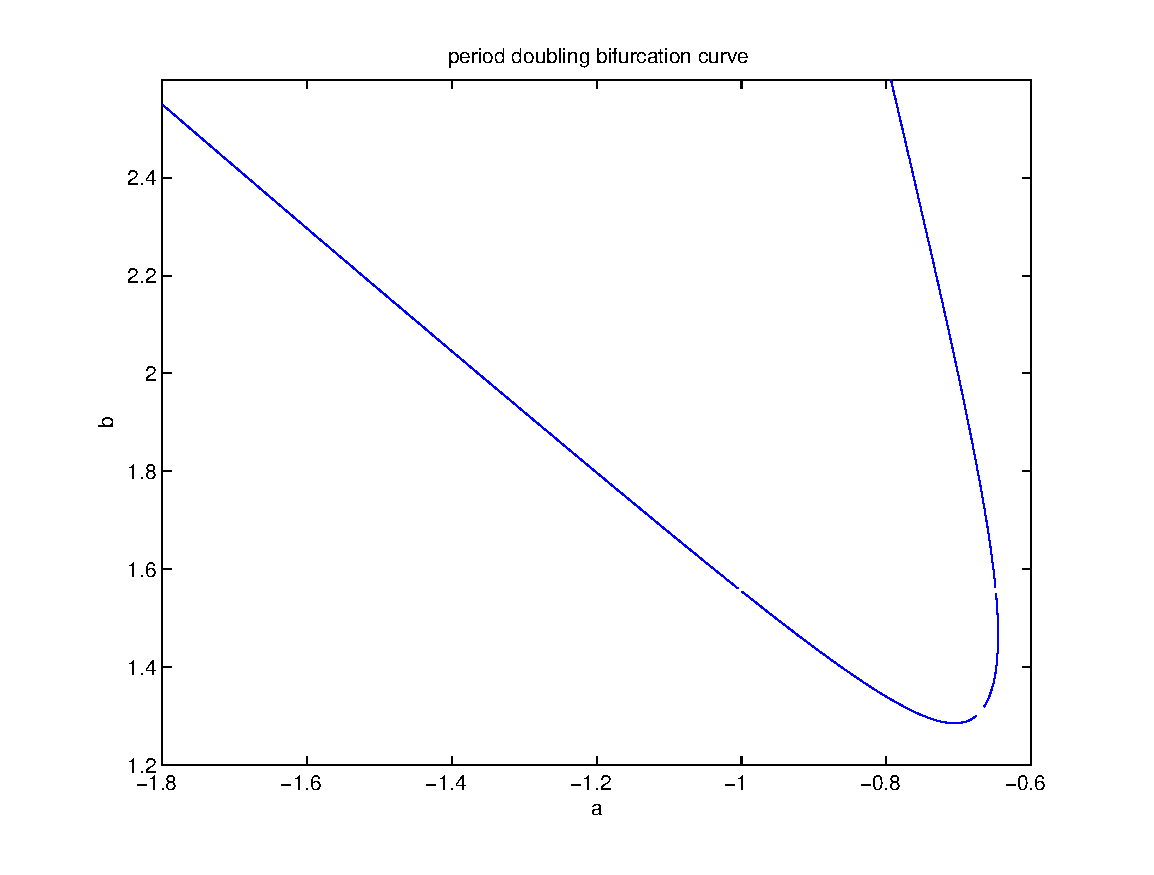
\includegraphics[scale=0.6]{fig/pdbif2.eps}
\end{center}
\caption{Period doubling bifurcation curve of the period-1 solution.}
\label{pdbif}
\end{figure}
Also, the arising period-2 orbits can be computed by switching to this new branch of solutions:
{ \small \begin{quote} \begin{lstlisting}[basicstyle=\tt,frame=single]
sys-glass.so            SYSNAME
112                     LABEL
14 P2 1 P0              TYPE, CP, NPARX, PARX ....
...
\end{lstlisting} \end{quote} } \noindent
%
\begin{figure}
\begin{center}
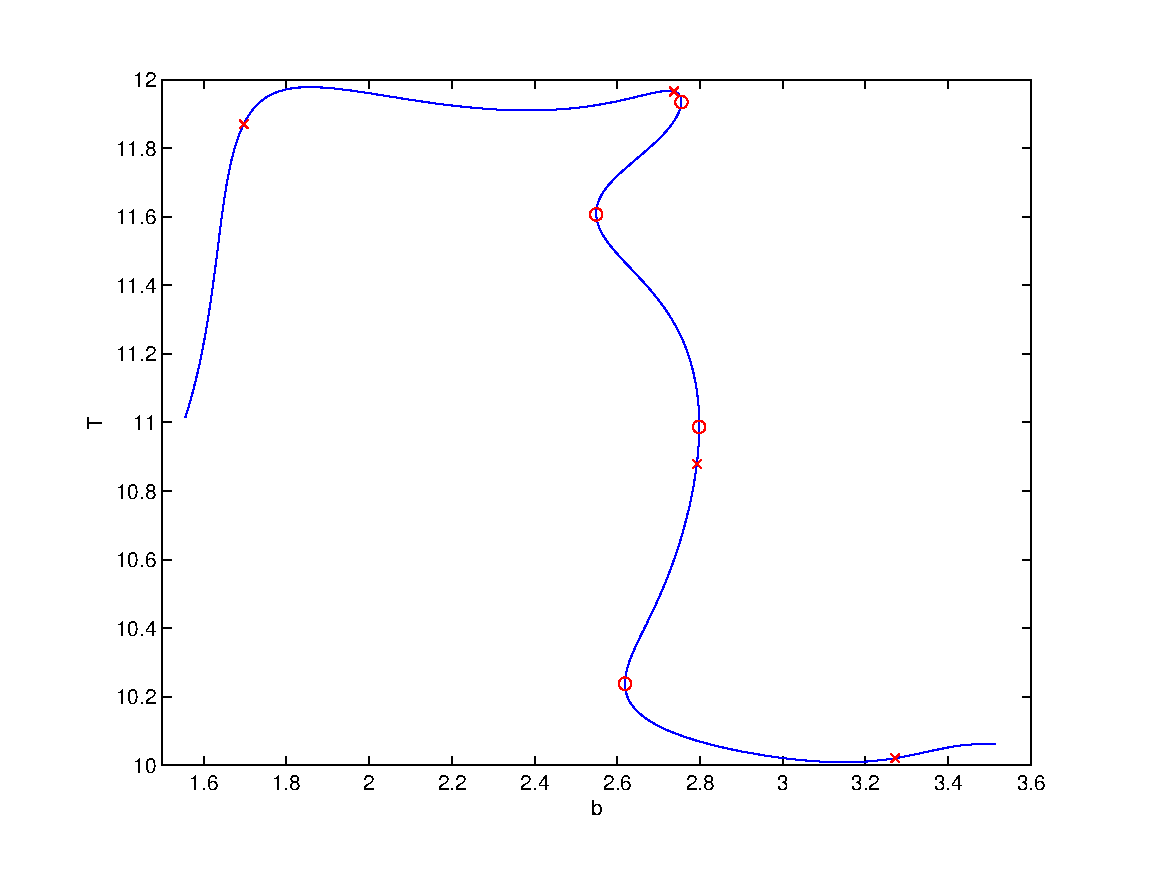
\includegraphics[scale=0.6]{fig/pdsw.eps}
\end{center}
\caption{The period-2 branch. Period doublings are denoted by $\times$, while $\circ$ refers to fold bifurcation. }
\label{pdsw}
\end{figure}
Figure \ref{pdsw} shows the bifurcation diagram of the period-2 orbit. Using the previous methods we continue the bifurcations on this period-2 branch, which gives a more detailed information about the solutions. A three dimensional bifurcation diagram can be seen in Fig.\ \ref{pdfold}, which shows the complicated orbit structure.
\begin{figure}
\begin{center}
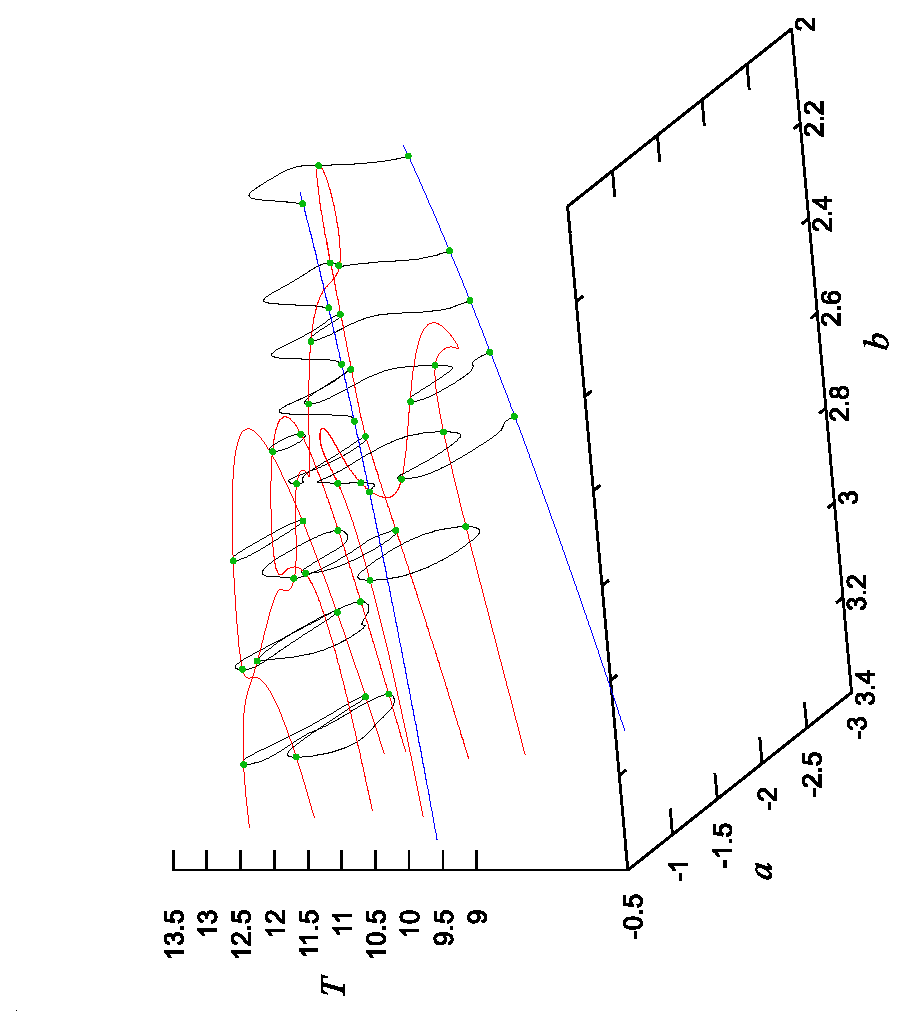
\includegraphics[scale=0.6,angle=270]{fig/fold3d-2.eps}
\end{center}
\caption{Fold bifurcations of the period-2 orbits. Black curves are periodic solutions continued along $b=$ constant lines. Red curves refer to fold bifurcations, while the blue line is the period doubling curve, where the period-2 orbits arise. }
\label{pdfold}
\end{figure}

\section{Algorithms used in the software}

The algorithms of this software are described in Szalai et al.\ \cite{szalai-cont}, with the exception of torus continuation. For continuation, the pseudo-arclength method is used (see \cite{handbook, tutorial1, tutorial2}). Periodic orbits are discretized by orthogonal collocation, which was also used in several other software packages. The stability and convergence of this method was proved by Engelborghs and Doedel \cite{engstab} (see also \cite{engcol}). Bifurcations are continued using the newly introduced characteristic matrices for periodic solutions \cite{szalai-cont}.

\subsection*{Acknowledgments}

The author is highly indebted to G\'abor St\'ep\'an (Budapest University of 
Technology and Economics) for his constant support. He is also
obliged to S.~John Hogan for partially supporting a 5 month visit at the University of Bristol.
This research was supported financially by a Hungarian E\"otv\"os Scholarship and a Fulbright grant.

\bibliographystyle{siam}
\bibliography{manual-bibl.bib} \label{sec:bibliography}


\end{document}
